\PassOptionsToPackage{xetex}{xcolor}
\PassOptionsToPackage{xetex}{graphicx}
\documentclass[a4paper,landscape,headrule,footrule,xetex]{foils}

%%% FIXME --- ask about why they like holmes

%%% FIXME --- ask which language they read it in

%%% FIXME --- ask which genre

%%
%%%  Macros
%%%
\newcommand{\logo}{~}
\MyLogo{HG8011 (2019)}
\newcommand{\Story}{\SHA{HOUN}{The Hound of the Baskervilles}}

\newcommand{\header}[3]{%
\title{\vspace*{-2ex} \large Detecting Meaning with Sherlock Holmes\thanks{Creative Commons Attribution License: you are free to share and adapt as long as you give appropriate credit and add no additional restrictions: 
\protect\url{https://creativecommons.org/licenses/by/4.0/}.}
%\footnotemark
\\[2ex] \Large  \emp{#2} \\ \emp{#3}}
\author{\blu{Francis Bond}   \\ 
\normalsize  \textbf{Division of Linguistics and Multilingual Studies}\\
\normalsize  \url{http://www3.ntu.edu.sg/home/fcbond/}\\
\normalsize  \texttt{bond@ieee.org}}
 \date{Location: LT25}
 \renewcommand{\logo}{#2}
 \hypersetup{
   pdfinfo={
     Author={Francis Bond},
     Title={#2},
     Subject={HG8011: Detecting Meaning with Sherlock Holmes},
     Keywords={Semantics, Pragmatics, Meaning},
     License={CC BY 4.0}
   }
 %  pdfcopyright={Copyright © Francis Bond. Creative Commons 4.0 Attribution License.}
 %  pdflicenseurl={http://creativecommons.org/licenses/by/4.0/}
 }
}
%%
%% Multilingual Stuff
%%
\usepackage[a4paper,landscape,margin=25mm]{geometry}

\usepackage{fontenc}
\usepackage{polyglossia}
\setmainlanguage{english}
\setmainfont{TeX Gyre Pagella}
\usepackage{xeCJK}
\setCJKmainfont{Noto Sans CJK SC}
\setCJKsansfont{Noto Sans CJK SC}
\setCJKmonofont{Noto Sans CJK SC}
%\setCJKttfont{Noto Sans CJK SC}
%\setCJKmainfont{WenQuanYi Micro Hei}
%\clearpage
%\setCJKmainfont{AR PL SungtiL GB}

\usepackage[xetex]{xcolor}
\usepackage[xetex]{graphicx}
\newcommand{\blu}[1]{\textcolor{blue}{#1}}
\newcommand{\grn}[1]{\textcolor{green}{#1}}
\newcommand{\hide}[1]{\textcolor{white}{#1}}
\newcommand{\emp}[1]{\textcolor{red}{#1}}
\newcommand{\txx}[1]{\textbf{\textcolor{blue}{#1}}}
\newcommand{\lex}[1]{\textbf{\mtcitestyle{#1}}}

\usepackage{pifont}
\renewcommand{\labelitemi}{\textcolor{violet}{\ding{227}}}
\renewcommand{\labelitemii}{\textcolor{purple}{\ding{226}}}

\newcommand{\subhead}[1]{\noindent\textbf{#1}\\[5mm]}

\newcommand{\Bad}{\emp{\raisebox{0.15ex}{\ensuremath{\mathbf{\otimes}}}}}
\newcommand{\bad}{*}

\newcommand{\com}[1]{\hfill \textnormal{(\emp{#1})}}%
\newcommand{\cxm}[1]{\hfill \textnormal{(\txx{#1})}}%
\newcommand{\cmm}[1]{\hfill \textnormal{(#1)}}%
\usepackage{amssymb}
\usepackage{relsize,xspace}
\newcommand{\into}{\ensuremath{\rightarrow}\xspace}
\newcommand{\ent}{\ensuremath{\Rightarrow}\xspace}
\newcommand{\nent}{\ensuremath{\not\Rightarrow}\xspace}
\newcommand{\tot}{\ensuremath{\leftrightarrow}\xspace}
\usepackage{url}
\usepackage[hidelinks]{hyperref}
\hypersetup{
     colorlinks,
     linkcolor={blue!50!black},
     citecolor={red!50!black},
     urlcolor={blue!80!black}
}
%\usepackage{hyperxmp}
\newcommand{\lurl}[1]{\MyLogo{\url{#1}}}

\usepackage{mygb4e}
\let\eachwordone=\itshape
\newcommand{\lx}[1]{\textbf{\textit{#1}}}
\newcommand{\ix}{\ex\it}

\newcommand{\cen}[2]{\multicolumn{#1}{c}{#2}}
%\usepackage{times}
%\usepackage{nttfoilhead}
\newcommand{\myslide}[1]{%
\foilhead[-25mm]{\raisebox{12mm}[0mm]{\emp{#1}}}%
\leftheader{}%
\MyLogo{\logo}}

\newcommand{\mytask}[1]{%
\foilhead[-25mm]{\raisebox{12mm}[0mm]{\emp{#1}}}
\leftheader{🔍 Hi}%
\MyLogo{\logo}}

\newcommand{\myslider}[1]{\rotatefoilhead[-25mm]{\raisebox{12mm}[0mm]{\emp{#1}}}}
%\newcommand{\myslider}[1]{\rotatefoilhead{\raisebox{-8mm}{\emp{#1}}}}

\newcommand{\section}[1]{\myslide{}{\begin{center}\Huge \emp{#1}\end{center}}}

\usepackage{tcolorbox}
% \newcommand{\task}{\marginpar{\raisebox{-1ex}{\large
%       \tcbox[colframe=red,colback=white,arc=3pt]{\textbf{?}}}}}
% \newcommand{\task}{\marginpar{\raisebox{-1ex}{
%       \hspace{-0.5em}\tcbox[colframe=red,colback=white,arc=3pt]{%
%         
\includegraphics[width=1.5em]{pics/detective}}}}}
\newcommand{\task}{\marginpar{\raisebox{-2ex}{
      \hspace{-0.5em}\reflectbox{
\includegraphics[width=2em]{pics/detective}}}}}

\usepackage[lyons,j,e,k]{mtg2e}
\renewcommand{\mtcitestyle}[1]{\textcolor{teal}{\textsl{#1}}}
%\renewcommand{\mtcitestyle}[1]{\textsl{#1}}
\newcommand{\chn}{\mtciteform}
\newcommand{\cmn}{\mtciteform}
\newcommand{\iz}[1]{\textup{\texttt{\textcolor{blue}{\textbf{#1}}}}}
\newcommand{\con}[1]{\textsc{#1}}
\newcommand{\gm}{\textsc}
\newcommand{\cmp}[1]{{[\textsc{#1}]}}
\newcommand{\sr}[1]{\ensuremath{\langle}#1\ensuremath{\rangle}}
\usepackage[normalem]{ulem}
\newcommand{\ul}{\uline}
\newcommand{\ull}{\uuline}
\newcommand{\wl}{\uwave}
\newcommand{\vs}{\ensuremath{\Leftrightarrow}~}
%%%
%%% Bibliography
%%%
\usepackage{natbib}
%\usepackage{url}
\usepackage{bibentry}


%%% From Tim
\newcommand{\WMngram}[1][]{$n$-gram#1\xspace}
\newcommand{\infers}{$\rightarrow$\xspace}



\usepackage{rtrees,qtree}
\renewcommand{\lf}[1]{\br{#1}{}}
\usepackage{avm}
%\avmoptions{topleft,center}
\newcommand{\ft}[1]{\textsc{#1}}
%\newcommand{\val}[1]{\textit{#1}}
\newcommand{\typ}[1]{\textit{#1}}
\avmfont{\sc}
%\avmvalfont{\sc}
\renewcommand{\avmtreefont}{\sc}
\avmsortfont{\it}


%%% From CSLI book
\newcommand{\mc}{\multicolumn}
\newcommand{\HD}{\textbf{H}\xspace}
\newcommand{\el}{\< \>}
\makeatother
\long\def\smalltree#1{\leavevmode{\def\\{\cr\noalign{\vskip12pt}}%
\def\mc##1##2{\multispan{##1}{\hfil##2\hfil}}%
\tabskip=1em%
\hbox{\vtop{\halign{&\hfil##\hfil\cr
#1\crcr}}}}}
\makeatletter

\newcommand{\sh}[1]{\lowercase{\href{https://fcbond.github.io/sh-canon/#1.html}}{#1}}
\newcommand{\SHA}[2]{\lowercase{\href{https://fcbond.github.io/sh-canon/#1.html}}{\textit{#2}}}


\begin{document}
\header{Lecture 9}{The Great Game: Sherlock in Popular Culture}%
{Sherlock Holmes and Herlock Sholmès}
\maketitle

%\include{schedule}


\myslide{Overview}

\begin{itemize}
\item The popularity of Sherlock Holmes
\item An Introduction to Copyright
\item Copyright and Sherlock Holmes
\item Transmission of information
\item Copyright and Lexicons
\item The Great Game
\end{itemize}


\section{The popularity of Sherlock Holmes}

\myslide{Sherlock Holmes Published Chronology}
%%%http://bakerstreet.wikia.com/wiki/Chronology_of_Sherlock_Holmes_Stories
\begin{itemize}\addtolength{\itemsep}{-1.5ex}
\item 1859: Doyle Born
\item 1887: \textit{A Study in Scarlet}
\item     1890: \textit{The Sign of the Four}
\item   July 1891 to December 1892: Stories that would make up \textit{The Adventures of Sherlock Holmes} published in 	\textit{The Strand} magazine
\item    December 1892 to November 1893: Stories that would make up \textit{The Memoirs of} Sherlock Holmes published in 	\textit{The Strand}   --- \emp{Break from Holmes}
\item    1901-2 (serial): \textit{The Hound of the Baskervilles}
\item    October 1903 to January 1905: Stories that would make up \textit{The Return of Sherlock Holmes} published in 	\textit{The Strand}
\item 1908–1913, 1917: Stories that would make up \textit{His Last Bow} (short stories) published.
\item     1914-15: \textit{The Valley of Fear}
\item  1921–1927: Stories that would become \textit{The Casebook of Sherlock Holmes} published. 
\item 1930: Doyle Dies
\end{itemize}

\myslide{Sherlock Holmes Internal Chronology}

\begin{itemize}\addtolength{\itemsep}{-1.5ex}
\item [1794]    Bow Street Runners formed (Britain's first police force)
\item [1829]    Metropolitan Police formed (at Great Scotland Yard)
\item [1852] 	John H. Watson is born (date derived from \sh{STUD})
\item [1854] 	Sherlock Holmes is born (date derived from \sh{LAST})
\item [1874] 	Holmes's first case, during the vacation after his second year of college
(\sh{GLOR})
\item [1891]  Sherlock Holmes dies (\sh{FINA}) --- \emp{the Great Hiatus}
\item [1894]  Just kidding --- he comes back, stronger than ever  (\sh{EMPT})
\item [1914]  \textit{His Last Bow} 	(\sh{LAST}) 

\end{itemize}
see
\href{http://blog.smartmemes.com/2010/03/sherlock-holmes-a-complete-chronology/}{Sherlock
  Holmes: a complete chronology} by Chris J Miller or
\href{http://webpages.charter.net/lklinger/Chrotabl.htm}{Life and
  Times of Mr. Sherlock Holmes, John H. Watson, M.D., Sir Arthur Conan
  Doyle, and Other Notable Personages} by Leslie Klinger for more
details.

\myslide{Popularity} 

\MyLogo{\$25,000 is \href{http://www.in2013dollars.com/1905-dollars-in-2015?amount=25000}{\$650,000 in current USD}, the highest sum ever
  paid to an author at the time \citep{Drake:2009}. }

\begin{itemize}\addtolength{\itemsep}{-1.8ex}
\item \textit{A Study in Scarlet} (\sh{STUD} 1887) was not so popular
\item The short stories, appearing in \textit{The Strand}, became very popular
\item Doyle preferred his historical fiction, in November 1891 he wrote to his mother: ``\textit{I think of slaying Holmes,... and winding him up for good and all. He takes my mind from better things.}'' %%%  Panek, LeRoy Lad (1987). An Introduction to the Detective Story. Bowling Green, OH: Bowling Green State University Popular Press. p. 78. ISBN 0-87972-377-7. Retrieved 4 January 2012.
 \\ His mother responded, ``\textit{You won't! You can't! You mustn't!}''
\item When he did kill off Sherlock Holmes in \textit{The Final Case}
  (\sh{FINA}) City of London stockbrokers donned black armbands, and
  some 20,000 angry readers canceled their Strand subscriptions!
\item The publication of \textit{The Hound of the Baskervilles}
  (\sh{HOUN}) was a huge success. Queues formed to buy copies and
  \textit{The Strand} had to go to a seventh printing for the only
  time in its history.
\item \textit{Collier's Weekly} in America offered such an enormous
  sum of money (\$25,000: \$650,000 in current USD) for new Holmes
  stories that Conan Doyle brought him back to life in \textit{The
    Adventure of the Empty House} (\sh{EMPT})
\item Doyle continued to write Holme's stories until 3 years before his death.
\end{itemize}

\myslide{Why were they so popular?}
\MyLogo{\citet{Drake:2009}}
\begin{itemize} \addtolength{\itemsep}{-1ex}
\item People liked Doyle's style
\item the stories were self-contained but featuring the same two main
  characters 
  \begin{itemize}
  \item you didn't have to worry about following the plot if you
    missed a story
  \item but there was still some continuity
  \item the relationship between Holmes and Watson was popular
  \item Holmes offers genius combined with quirky independence
  \item Watson is sensible, generous, kind, loyal and decent
  \end{itemize}
\item the cost of paper had fallen due to cheap imported wood-pulp
\item  printing presses were more  sophisticated and ran faster
\item the 1870 Education Act meant more people could read
\item reduced working hours introduced the notion of leisure time
\end{itemize}

People had time to read and wanted to: each month queues formed at the
news-stands on the day that the Strand Magazine was due to appear



\myslide{Adaptions: Plays}


\begin{itemize} \addtolength{\itemsep}{-1ex}
\item Doyle tried to write a play, but it was turned down 
\item William Gillette (actor and playwright) rewrote it: taking
  elements from several stories and adding a love interest (Alice
  Faulkner) and naming the page boy (Billy).
\item The play opened in New York in 1899 
  \begin{itemize}
  \item it ran there for more than 260 performances; then toured the United States
  \item then on to  London's Lyceum Theatre in 1901 for 200 performances
    \\ (a thirteen-year-old Charlie Chaplin played Billy the pageboy)
  \item the show was revived in 1905, 1906, 1910, and 1915
  \item The play introduces \eng{Elementary, my dear Watson}, and
    popularizes the deerstalker hat 
    and the curved pipe as Holmes props.
  \end{itemize}
\item Doyle then wrote his own (successful) adaptation of \sh{SPEC}
  \newpage
\item In 1916, a silent film was made, featuring  William Gillette
  \begin{itemize}
  \item it has been called "the most elaborate of the early movies".
  \item  a print of the (lost) film was found in the Cinémathèque Française's in 2014
\item You can see it at the
  \href{https://archive.org/details/SherlockHolmes1916}{Internet Film Archive}
  \end{itemize}
\end{itemize}

\myslide{Adaptions: Films}

\begin{itemize}
\item Guinness World Records lists Holmes as the "most portrayed movie
  character": more than 70 actors in over 200 films.
\item The first screen appearance was in the 30-second 1900 Mutoscope film: \textit{Sherlock Holmes Baffled}
\item New films appeared almost every year since then 
\item Basil Rathbone appeared in 14 films, starting with \sh{HOUN} in 1939
\item Robert Downey, Jr. (2009, 2011)
\item Ian McKellen (2015) \textit{Mr. Holmes}
\item   Henry Cavill (2020) \textit{Enola Holmes}
\end{itemize}

\myslide{Adaptions: TV}
\begin{itemize}
\item Jeremy Brett appeared in \textit{The Adventures of Sherlock Holmes}
  \begin{itemize}
  \item Granada Television films made between 1984 and 1994
  \item 41 episodes
  \item He had previously appeared as Watson with Charleton Heston as Holmes in \textit{The Crucifer of Blood} (1980)
  \item Often thought of as one of the greatest portrayals
  \end{itemize}
\item Benedict Cumberbatch appears in \textit{Sherlock} (2010–2017) 
\item Jonny Lee Miller 	appears in \textit{Elementary} 	(2012–present) with Lucy Liu as Joan Watson
\end{itemize}



% \section{Pastiches, Fan-fiction and more}

\myslide{Holmes in America}

\begin{itemize}
\item In the 19th century, England produced more books than America
  \begin{itemize}
  \item American copyright laws only protected American authors
  \item Before 1891 there was no protection at all
  \item After 1891, foreign authors could claim copyright and if a
    book was published in the US, then it could not be imported
  \end{itemize}
\item So the first two novels could be printed by anybody!
  \begin{itemize}
  \item Many, many editions came out
  \end{itemize}
\item Subsequent books had fewer variants (but were often pirated)
\end{itemize}

\myslide{Transformation}

\begin{itemize}
\item Consider \sh{SIGN}: It came out as
  \begin{itemize}
  \item \textit{The Sign of Four} \hfill (original)
  \item \textit{At the Sign of the Four}
  \item \textit{Sign of the Four}  
  \item \textit{A Sign of Four}
  \item \textit{Sherlock Holmes and the Sign of the ``4''}
  \item \textit{Sherlock Holmes and the Great Agra Treasure}
  \end{itemize}
\item[?] Which words change most: content words or function words? \task
\item The texts change for several reasons:
  \begin{itemize}
    \item British/American spelling differences
    \item Type setting errors
    \item Differing punctuation styles
    \item Different paragraph breaks
  \end{itemize}
\end{itemize}

\myslide{What changed in \sh{SIGN}?}
\MyLogo{\citep{Redmond:1990}}

\begin{tabular}{lll}
  Original & Variant & Comment \\
\hline
  Tabaccoes & Tabbaccos & UK/US \\
  Cold Harbour &  Cold Harbor & UK/US \\
  halloo & hallo  & UK/US \\
  card-board & cardboard & hyphenation \\
  mild balsmic & balsamic & error \\
  poured our & poured out & error (r/t)\\
  personal & persoual & error (n/u)\\
  wished & w shed & error (dropped i)\\
  This is not & That is not & change \\
  whiskey-and-soda & whisky and soda &  UK/US, hyphenation \\
\end{tabular}

Also many more differences in commas/dashes/semicolons (40),
hyphenation (5),  paragraph breaks (12), \ldots .


\myslide{What happens when you keep copying?}
\MyLogo{\citep[90,94]{Redmond:1990}}
Consider 6 different editions of \sh{SIGN}, each based on the one before

\begin{tabular}{lrrr}
  Edition & Year & Variation & \% increment \\
\hline
  Lippincot          & 1890 & 0   & 0.000 \\ 
  Waverly            & 1893 & 24  & 0.059 \\
  United States Book & 1893 & 36  & 0.029 \\
  Weeks              & 1894 & 113 & 0.100 \\
  Munro              & 1896 & 163 & 0.210 \\
  Books, Inc         & 1922 & 219 & 0.136 \\
  Kingsport Press    & 1923 & 233 & 0.034 
\end{tabular}

\begin{itemize}
\item The quality of the text (the signal) degrades.
\item A well known problem with analog transmission
\item Which is why we move to digital records
\end{itemize}


\section{Copyright and Licensing}

\myslide{Copyright}
\MyLogo{I am not a lawyer}
\begin{itemize}
\item Governments grant certain rights to authors of creative works,
  typically called \blu{copyrights} in order to encourage them
  to produce more
  \begin{itemize}
  \item The most basic right is the right to forbid people from
    copying it without permission
  \item Any work produced is by default copyright of the author
  \end{itemize}
\item Some or all of these rights can be waived or transferred
  \begin{itemize}
  \item An author may sell the rights for a manuscript to a publisher
  \item A blogger may place their postings in the public domain
  \item A publisher may give permission to an author to post their
    paper on their website
  \item A work may be distributed under a license that allows copying only under some conditions
  \end{itemize}

\item[*]  Renumeration was clearly important to Doyle: he wrote for money, and
  he kept writing for money  --- copyright makes it easier to be paid

\newpage
\item Copyright is relatively recent: the British Statute of Anne
  1710, \textit{An Act for the Encouragement of Learning, by
  vesting the Copies of Printed Books in the Authors or purchasers of
  such Copies, during the Times therein mentioned} was the first
  copyright statute, although cities, popes and royal families had
  granted limited monopolies earlier.
  \begin{itemize}
  \item Before printing, copyright was not really necessary
  \item It was very much connected to censorship and control of information
  \item It originally applied only to books, but now is applied much
    more widely: translations, maps, performances, paintings,
    photographs, films, programs, \ldots
  \end{itemize}
\item Copyright laws are national laws, although they may be
  harmonized by treaties
  \begin{itemize}
  \item A text may be illegal to copy in one country, but legal in another
  \end{itemize}
\newpage
\item Copyright laws change over time
  \begin{itemize}
  \item E.g. in the U.S. originally 14 years for books only
  \item Now 70 years after the death of the author for almost
    everything \\ (but not recipes or fashion!)
  \end{itemize}
\item New technology complicates things
  \begin{itemize}
  \item Sending email involves making multiple copies on different servers
  \item Recording speech can happen without the creator's knowledge
  \end{itemize}
\item[*] International copyright was important to Doyle --- it was
  American publishers who paid the advance for \sh{HOUN}

\end{itemize}


\myslide{But copyright also restricts}

\begin{itemize}
\item Many translations and pastiches flourished --- current copyright
  laws would stop them
\item Copyright on most of the stories stopped in the year 2000, so
  Holmes is now in the public domain (except the last few stories in the US)
\item This is one of the factors that has enabled the recent flood of
  new Holmes-based films and TV (and books)
  \begin{itemize}
  \item it costs nothing to use the characters
  \item you can make changes to them without asking for permission to
    the copyright holder
  \end{itemize}
\item It was one of the reasons I chose the texts for my research
\item Lack of copyright allows people to use, enjoy and extend the stories and characters
\end{itemize}


\begin{center}
  \emp{Copyright issues are very complicated}
\end{center}

\myslide{Some Rough Guidelines}

\begin{itemize}
\item Copying something which is under copyright is \blu{illegal} unless
  specific permission is granted or it falls under \textbf{fair
    dealing}, such as for the purpose of research or education
\item How can you get permission?
  \begin{itemize}
  \item You can buy it (for some works)
  \item You can get signed permission from the copyright holder
\\ (or recorded permission for preliterate speakers)
  \item You can get implicit permission (e.g. for email or web pages)
  \item It can be permitted by a license
    \begin{itemize}
    \item \txx{CC-by} allows you to copy and redistribute if you acknowledge
    \item \txx{CC-by-nc} allows you to copy and redistribute if you
      acknowledge and it is for non-commercial use
    \end{itemize}
  \end{itemize}

\newpage \lurl{http://en.wikipedia.org/wiki/Fair_dealing}
\item The following factors will be considered to decide if it is fair
  dealing (in Singapore)
  \begin{itemize}
  \item  purpose and character of the dealing, including whether such dealing is of a commercial nature or is for non-profit educational purposes
  \item  nature of the work or adaptation
  \item amount copied, relative to the whole work
  \item  effect of the dealing upon the potential market for the work, and effect upon its value
  \item the possibility of obtaining the work or adaptation within a reasonable time at an ordinary commercial price
  \item whether the copy is for the purpose of criticism or review; for the purpose reporting of news; for the purpose of judicial proceedings or professional advice (a sufficient acknowledgment of the work is required)
  \item it is not an infringement if a person makes a copy from an
    original copy of a computer program  as a back-up
  \end{itemize}
\end{itemize}

\myslide{Copyright for Corpora}
\MyLogo{}
\begin{itemize}
\item Arguments for \blu{restrictive licensing}
  \begin{itemize}
  \item Competitive advantage (common for speech corpora)
  \item Compensation for the effort of creation
  \item Minimize effect on the value of the original work
  \end{itemize}
\item Arguments for \blu{open licensing}
  \begin{itemize}
  \item Annotation is expensive: making the data open gets the best
    return on this investment
  \item Annotation is typically ongoing: opening the data gets you
    more feedback
 \item Researchers are evaluated by the impact that their work has: open data generally has more impact.
  \item Language data is part of our shared heritage
  \end{itemize}
\end{itemize}

\myslide{Choice of License if you create data}
\begin{itemize}
\item Should be considered early on (before you start compiling your data)
\item May depend on the funding body
\item Depends on the source data
\item General trend is to open licensing
  \begin{itemize}
  \item Open Science Project
  \item Open Access Journals
  \item Open Source Software
  \end{itemize}
\item Try to chose a standard license (such as Creative Commons)
\item \href{http://research.ntu.edu.sg/rieo/RI/Pages/Research-Data-Policies.aspx}{NTU's policy}: ``The final research data from projects carried out
  at NTU shall be made available for sharing (via the NTU Data
  Repository) unless there are prior formal agreements with external
  collaborators and parties on non-disclosure or proprietary use of
  the data.''  NTU's default license is CC-BY-NC 

\end{itemize}

\myslide{Creative Commons Licenses}
\lurl{http://creativecommons.org/licenses/}
\medskip
\begin{tabular}{lccc}
  License       & Derivative Works & Same License & Commercial Use \\
\hline
  CC-BY         &   + &  - &  + \\
  CC-BY-SA      &   + &  + &  + \\  
  CC-BY-NC      &   + &  - &  - \\
  CC-BY-ND      &   - &  - &  + \\
  CC-BY-NC-SA   &   + &  + &  - \\
  CC-BY-NC-ND   &   - &  - &  - \\
\end{tabular}
\begin{description} \addtolength{\itemsep}{-0.5ex}
\item[BY] Attribution (all licenses)
\item[SA] Share Alike (requires copies to have the same license)
\item[NC] Non-Commercial \com{\href{https://opendefinition.org/}{Not Open}}
\item[ND] No Derivatives (allows only exact copies) \com{\href{https://opendefinition.org/}{Not Open}}
\end{description}

Many, many other license also exist (GPL, MIT, BSD, Apache, \ldots)

 \myslide{The Open Definition}
\MyLogo{https://opendefinition.org/}
 \begin{itemize}
 \item The Open Definition sets out principles that define \txx{openness}
   in relation to data and content.
 \item It makes precise the meaning of \txx{open} in the terms \txx{open data}
   and \txx{open content} and thereby ensures quality and encourages
   compatibility between different pools of open material.
 \item It can be summed up in the statement that:
   \begin{quote}
     “Open means anyone can freely access, use, modify, and share for
     any purpose (subject, at most, to requirements that preserve
     provenance and openness).”
   \end{quote}
 \item Put most succinctly:
   \begin{quote}
     “Open data and content can be freely used, modified, and shared
     by anyone for any purpose”
   \end{quote}
 \end{itemize}
% \begin{center}
%   Be careful of copyright
% \end{center}


% Sherlock Holmes was so popular that he was incorporated into other stories

% In Arsene Lupin

% (as was common in folk tales)  <--- check with Jane/Sam

% More stories created in e.g. German

%%% FIXME copyright issues https://www.techdirt.com/articles/20150524/17521431095/sherlock-holmes-case-never-ending-copyright-dispute.shtml

\section{Spreading Overseas }

\myslide{Transmission}

\begin{itemize}
\item Writers are also readers and translators are both
\item They read, often in multiple languages
\item This can inspire new works
\item Holmes was partially inspired by Edgar Allan Poe's (1809–1849)
  ``C. Auguste Dupin'' a detective even before we had the word!
\item Often people imitate style and even reuse characters
  \begin{itemize}
  \item  \txx{pastiche} ``a work of art that imitates the style of some previous work''
  \item \txx{fanfic} ``Amateur fiction created by fans, incorporating the characters and concepts another work, typically without permission from the author or owner''
  \end{itemize}
\item We will also look at this in week 12 \textit{Holmes in Translation}.
\end{itemize}

\myslide{Sherlock Holmes and Herlock Sholmès}
\MyLogo{Arsene Lupin is of course the grandfather of LUPIN III, the world's number one thief. ルパン,  ルパン!}

\begin{itemize}
\item The \textit{Arsène Lupin} stories were written in French by
  Maurice Leblanc (1864–1941).
\item They appeared from 1905 to 1939.
\item In the 1906 story \textit{Sherlock Holmes Arrives Too Late} an
  aged Holmes meets a young Lupin for the first time.
\item Conan Doyle objected to the use of the name, and when the
  stories were collected in a book, the English detective \emp{Herlock
  Sholmes} appeared instead.
\item He appeared in two more stories.
\item When they were translated into English and published in the US
  in 1910, the names were further changed to \emp{Holmlock Shears}
  and his assistant \emp{Wilson}.

\end{itemize}



\myslide{The books}



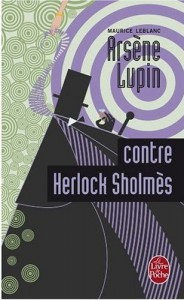
\includegraphics[height=0.7\textheight]{pics/arsene-lupin-vs-herlock-sholmes1-184x300.jpg}
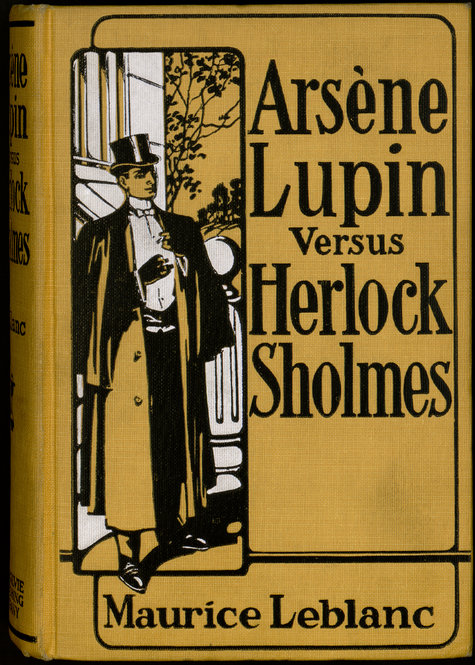
\includegraphics[height=0.7\textheight]{pics/as-vs-hs}
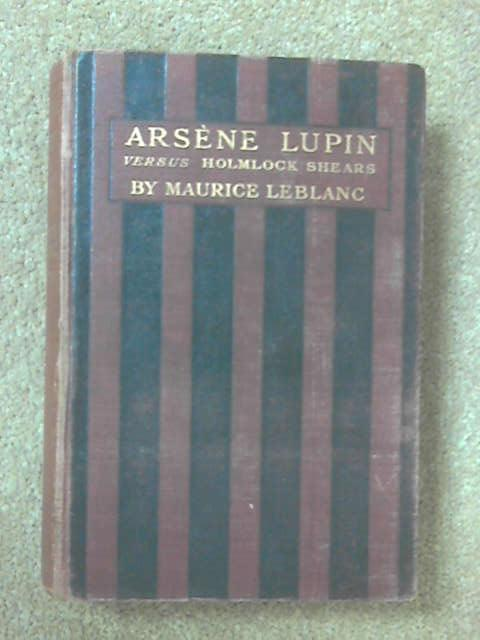
\includegraphics[height=0.7\textheight]{pics/lupi.jpg}


\myslide{Harry Dickson (i)}
\MyLogo{Much information from 
\href{https://en.wikipedia.org/wiki/Harry_Dickson}{Wikipedia:Harry Dickson}}

\begin{itemize}
\item A series of 230 cheap pulp novels ran from 1907 to 1911 in Germany.
  \begin{itemize}
  \item The first ten had Holmes as the hero, with the series title
    \textit{Detective Sherlock Holmes und seine weltberühmten
      abenteuer} ``Sherlock Holmes' Most Famous Cases''
  \item Fearing legal issues the series was changed to \textit{Aus dem
      Geheimakten des Weltdetektivs} ``The Secret Files of the King
      of Detectives''; Holmes was still the hero, but his side kick
      was Harry Taxon.
    \end{itemize}
  \item These were translated in French as \textit{Les Dossiers
      Secrets de Sherlock Holmes} ``Sherlock Holmes' Secret Files''
    but changed from issue 2 to \textit{Les Dossiers Secrets du Roi
      des Détectives} ``The Secret Files of the King of Detectives''
  \item The German series was translated/adapted into Dutch as
    \textit{Harry Dickson de Amerikaansche Sherlock Holmes} ``Harry
    Dickson, the American Sherlock Holmes'', with assistant Tom Wills.
    The Dutch series lasted 180 issues, until May 1935.
    
  \end{itemize}

\myslide{Harry Dickson (ii)}
\MyLogo{Much information from 
\href{https://en.wikipedia.org/wiki/Harry_Dickson}{Wikipedia:Harry Dickson}}

\begin{itemize}
\item A Belgian publisher asked writer Jean Ray to translate the Dutch
  series into French: \textit{Harry Dickson, le Sherlock
  Holmes Americain} began in January 1929.
\item Ray thought the original stories mediocre and asked permission
  to rewrite them.  The publisher agreed, provided only that each
  story be about the same length as the original, and match the book's
  cover illustration!
\item The series has 178 issues in all (1929--1938)
\item The stories are set in the 1920s and 1930s.
\item The stories are far more fantasy-oriented than the true
  Holmesian canon.  Villains include Professor Flax 'the human
  monster', mummies, Hanuman, Medusa, \ldots
\item Harry Dickson's fame in France rivals that of Sherlock Holmes and Arsène Lupin.
\end{itemize}



\myslide{Holmes in Turkey}
\MyLogo{\citep{Toury:1995,Tahir-Gürçağlar:2008}}
% Toury, Gideon. 1995. Descriptive translation studies and beyond. Amsterdam: John Benjamins.
\begin{itemize}\addtolength{\itemsep}{-1ex}
\item Holmes' stories were also popular in Turkey, where in addition
  to stories by Doyle, the Harry Taxon/Harry Dickson stories were
  widely translated
\item Many \txx{pseudo-translation}s flourished ``texts which have
  been presented as translations with no corresponding source texts in
  other languages ever having existed''
\item In one series \textit{Sherlock Holmes'in Metresi} ``Sherlock
  Holmes's Mistress'', he is a bumbling detective and his mistress Miss
  Barclay solves the mystery.
\item He also appears as a character in a popular local crime series: Cingöz Recai ``Recai the Shrewd'' in \textit{Şerlok Holmes'e Karşı Cingöz Recai} ``Sherlock Holmes vs Cingöz Recai''
\item Two series ``The famous English Police Inspector Sherlock Holmes
  Series'' (83 dime novels 1944--1945) and ``Sherlock Holmes'
  Wonderful Adventures'' (85 16-page stories) contained a mixture of
  cut-down versions of the original stories and new stories.
\item Most of these books were published with neither author or
  translator shown
\end{itemize}

\myslide{The books}


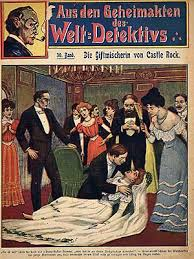
\includegraphics[height=0.7\textheight]{pics/weldetektives.jpeg}
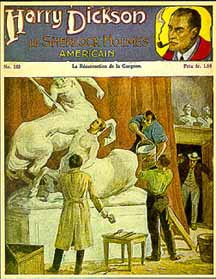
\includegraphics[height=0.7\textheight]{pics/harrydickson1.jpg}
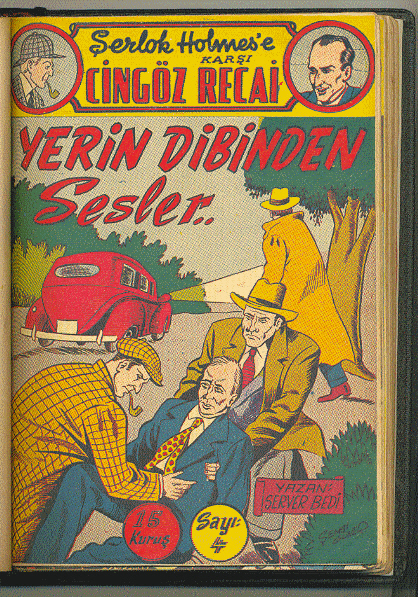
\includegraphics[height=0.7\textheight]{pics/yerindibindensesler.jpg}

\myslide{Summary}

\begin{itemize}
\item Sherlock Holmes was very, very popular
\item There are more Holmes stories written by other authors than by Doyle
\item Stories inspire other stories
\item Copyright laws attempt to balance the benefits to the authors
  and the benefit to society
  \begin{itemize}
  \item Strict copyright gets authors (publishers) money for longer
  \item Strict copyright enables people to create more
  \item Loose copyright allows authors/translators more freedom
  \item Loose copyright allows consumers access to more
  \item There are copyright exceptions (research/parody/review/indexing)
  \item Big data analysis often ignores copyright
  \end{itemize}
\end{itemize}


\section{Copyright and Lexicons}


\myslide{Who owns language?}
\MyLogo{\citep{Alberts:Jooste:2012}}
\begin{itemize}\addtolength{\itemsep}{-1ex}
\item You can't copyright facts: e.g. the weight of an electron
\item Is a dictionary definition a fact?
  \begin{itemize}
  \item \lex{dog} ``a member of the genus Canis (probably descended
    from the common wolf) that has been domesticated by man since
    prehistoric times; occurs in many breeds''
  \end{itemize}
\item The definition shows some creativity
\item[?] Can you come up with a better definition? \task 
\item[?] Are some words easier to define and why? \task 


\newpage
\item What part-of-speech a word is, how it is translated,
  collocations it appears in and declensions and variant spellings 
  almost certainly can not be copyrighted

\item The choice of which words to put in, format, division into senses (the \txx{macrostructure}) can probably be copyrighted
\item The wordings of definitions can also probably be copyrighted,
  but there is a long tradition of following earlier definitions quite closely
\item Terminology shows less creativity
\\
``It is highly unlikely that even the fine-tuned expert
  definitions found in national and international standards would
  qualify as \ldots\ unique expression.  Standard definitions are
  frequently reused in other standards, in general and technical
  texts, and in terminology databases'' Wright (1996: 2), cited in
  \citet{Alberts:Jooste:2012}
\item Examples cited in dictionaries are normally so short as to not
  be protected by copyright --- standard practice is to never ask for permission to cite them, but to properly cite them \citep{Landau:1989}
\end{itemize}

\section{The Great Game}


\myslide{The Sherlockian Game}
\MyLogo{Much information from 
\href{https://en.wikipedia.org/wiki/Sherlockian_game}{Wikipedia:Sherlockian Game}}
\begin{itemize}
\item The Great Game (aka the Sherlockian game, the Holmesian game) is
  the pastime of attempting to resolve anomalies and clarify implied
  details about Sherlock Holmes and Dr. Watson using the canon.
\begin{itemize}
\item \lex{canon} ``a collection of books accepted as holy scripture
  especially the books of the Bible recognized by any Christian church
  as genuine and inspired''
\item It is common to distinguish between the \lex{canon} and \lex{apocrypha} ``14 books of the Old Testament included in the Vulgate (except for II Esdras) but omitted in Jewish and Protestant versions of the Bible; eastern Christian churches (except the Coptic Church) accept all these books as canonical; the Russian Orthodox Church accepts these texts as divinely inspired but does not grant them the same status''
\item The canon of Sherlock Holmes consists of the 56 short stories
  and four novels written by Sir Arthur Conan Doyle
\end{itemize}
\item The great game treats Holmes and Watson as real people and uses
  aspects of the canonical stories combined with the history of the
  era of the tales' composition to construct fanciful biographies of
  the pair.
\end{itemize}

\myslide{Studies in the Literature of Sherlock Holmes}
\MyLogo{\href{http://www.diogenes-club.com/studies.htm}{Monsignor Ronald A. Knox (1911)}}

This was the essay that sparked things off:

\begin{quotation}

  \eng{There is, however, a special fascination in applying this
    method to Sherlock Holmes, because it is, in a sense, Holmes's own
    method.  `It has long been an axiom of mine,' he says, `that the
    little things are infinitely the most important.' It might be the
    motto of his life's work.  And it is, is it not, as we clergymen
    say, by the little things, the apparently unimportant things, that
    we judge of a man's character.}


  \eng{If anyone objects, that the study of Holmes literature is
    unworthy of scholarly attention, I might content myself with
    replying that to the scholarly mind anything is worthy of study,
    if that study be thorough and systematic.  But I will go further,
    and say that if at the present time we need a far closer
    familiarity with Sherlock's methods. }
\end{quotation}
\newpage 
\begin{quotation}
\eng{There is a special kind of epigram, known as the Sherlockismus, of which the indefatigable Ratzegger has collected no less than one hundred and seventy-three instances.  The following may serve as examples:}
\end{quotation}

\begin{flushleft}
  \eng{`Let me call your attention to the curious incident of the dog in
  the night-time.' \\
 `The dog did nothing at all in the night-time.'\\
  `That was the curious incident,' said Sherlock Holmes.\\
\bigskip
  And again:
\bigskip
\\  `I was following you, of course.' 
\\ `Following me?  I saw nobody.'
\\  `That is what you must expect to see when I am following you,' said
  Sherlock Holmes.}
\end{flushleft}

\begin{quotation}
\eng{To write fully on this subject would need two terms' lectures at least.  Some time, when leisure and enterprise allow, I hope to deliver them.  Meanwhile, I have thrown out these hints, drawn these outlines of a possible mode of treatment.  You know my methods, Watson: apply them.}

  \end{quotation}

\myslide{Some examples}

\begin{itemize}
\item[?] Did anyone notice any hard-to-interpret things in \sh{SPEC}, \sh{DANC} and \sh{REDH}? \task
 %%% Baboons and Cheetahs are not from Africa
 %%% There is no such snake as the swamp adder
 %%% it takes place in the autumn, specifically October 1890, yet the advertisement for the Red-headed League supposedly appeared "just two months ago" on 27 April. 
\end{itemize}

\myslide{Dr. Watson's Christian Name}
\MyLogo{From \textit{Unpopular Opinions} \citep{Sayers:1947}.  I also recommend the essays \textit{Are Women Human?} and \textit{The Abomination of Braces}.}

\begin{itemize} \addtolength{\itemsep}{-0.5ex}
\item Watson's name is \emp{John H. Watson}
\\ ``\eng{Somewhere in the vaults of the bank of Cox and Co., at Charing Cross, there is a travel-worn and battered tin dispatch-box with my name, \ul{John H. Watson}, MD, Late Indian Army, painted upon the lid.}'' \sh{THOR}
\item But in \textit{The Man with the Twisted Lip} (\sh{TWIS}) his wife, Mary Morstan, refers to him as James! 
\\ ```\eng{It was very sweet of you to come. Now, you must have some wine and water, and sit here comfortably and tell us all about it. Or should you rather that I sent \ul{James} off to bed?}''
\item Rejecting the possibility of a misprint, Sayers discovers a possible solution:
  \begin{itemize}
  \item \eng{Hamish} is a masculine given name in English
  \item It is the Anglicised form of the vocative case of the Scottish Gaelic \lex{Seumas}: \eng{Sheumais}.
  \item The Scottish Gaelic \eng{Seumas} is the equivalent to the English
    \eng{James}
  \end{itemize}
\item So his middle name is Hamish, but Mary Anglicizes it to James.

\end{itemize}


\myslide{Indian Animals}

\begin{itemize}
\item In \sh{SPEC},  we are told ``\eng{He has a passion also for Indian animals, which are sent over to him by a correspondent, and he has at this moment a cheetah and a baboon, which wander freely over his grounds, and are feared by the villagers almost as much as their master.}''
\item But Baboons and Cheetahs come from Africa
\item For the story it doesn't matter: exotic animal is exotic animal
\item The story was written early on, when Doyle had just returned to
  London, was not very wealthy and did not have easy access to
  libraries
\item You can see it as a problem of information access or of how we
  treat otherness
\item[?] Can you come up with an explanation that works in canon? \task


\end{itemize}

\myslide{Summary}

\begin{itemize}
\item Fanfiction, fan wikis, and fandom in general are often looked down upon
\item But they have a long and distinguished history
\item Many respected novelists have borrowed characters from each other
\item Many respected novelists are geeks
\item Studying something minutely helps one to do it better
\end{itemize}



\myslide{Father Knox's Ten Commandments}
\MyLogo{\citet{Knox:1929}}

\begin{itemize}   % \addtolength{\itemsep}{-1ex}
\item[I.]     The criminal must be someone mentioned in the early part of the story, but must not be anyone whose thoughts the reader has been allowed to follow;
\item[II.]    All supernatural or preternatural agencies are ruled out as a matter of course;
\item[III.]   No more than one secret room or passage is allowable.  I would add that a secret passage should not be brought in at all unless the action takes place in the kind of house where such devices might be expected;
\item[IV.]   No hitherto undiscovered poisons may be used, nor any appliance which will need a long scientific explanation at the end;
\item[V.]    No Chinaman must figure into the story;\footnote{In Msgr. Knox's time, one of the most overused plot mechanisms was the introduction of "a Chinaman" or other foreign, exotic or otherwise unusual character from "another land" as the malefactor.  This comment was not intended as a "racist" one, but as a reaction to this plotting mechanism.}
\end{itemize}
\newpage

\begin{itemize}\addtolength{\itemsep}{-0.5ex}
\item[VI.]   No accident must ever help the detective, nor must he ever have an unaccountable intuition which proves to be right;
\item[VII.]  The detective must not, himself, commit the crime;
\item[VIII.] The detective must not light on any clues which are not
  instantly produced for the inspection of the reader;
\item[IX.] The stupid friend of the detective, the Watson, must not
  conceal any thoughts which pass through his mind; his intelligence
  must be slightly, but only very slightly, below that of the average
  reader;
\item[X.] Twin brothers, and doubles generally, must not appear unless
  we have been duly prepared for them
\end{itemize}

Created as a set of bylaws for the
\href{https://en.wikipedia.org/wiki/Detection_Club}{Detection Club}
(which included G. K.  Chesterton, Emma Orczy, Dorothy L. Sayers,
Anthony Cox, Agatha Christie) these Ten Commandments served as a codex
for the Club as well as a general code for the writing of detective
fiction: Conan Doyle frequently broke them.


\small
\bibliographystyle{aclnat}
\bibliography{abb,mtg,nlp,ling}

\end{document}

%%% Local Variables: 
%%% coding: utf-8
%%% mode: latex
%%% TeX-PDF-mode: t
%%% TeX-engine: xetex
%%% End: 

